%! TeX program = xelatex

\documentclass[12pt, a4paper]{article}
\usepackage{cmap}
\usepackage[fontsize=12pt]{scrextend}
\usepackage[T2A]{fontenc}
\usepackage[utf8]{inputenc}
\usepackage[english,russian]{babel}
\usepackage{amsmath,amsfonts,amssymb,amsthm,mathtools}
\usepackage[left=20mm, top=20mm, right=20mm, bottom=20mm, nohead, footskip=1cm]{geometry}
\usepackage{multirow}
\usepackage{array}
\usepackage{multicol}
\usepackage{graphicx}
\usepackage{wrapfig}
\usepackage{indentfirst}
\usepackage{enumitem}

\usepackage{polyglossia}
\usepackage{titlesec}
\usepackage{sectsty}
\usepackage{setspace}
\usepackage{fontspec}
\defaultfontfeatures{Mapping=tex-text}

\usepackage{lipsum}
\usepackage{tocloft}
\usepackage[dvipsnames]{xcolor}

\usepackage{caption}
%\captionsetup{labelfont=it, textfont=it}
%\captionsetup[figure]{name=Схема}

\usepackage{hyperref}

\hypersetup{
    colorlinks=false,
    linktoc=all
}
\urlstyle{same}

\setmainlanguage{english}
\setotherlanguage{russian}
\setkeys{russian}{babelshorthands=true}
\setmainfont{Times New Roman}
\newfontfamily\cyrillicfont{Times New Roman}
\let\cyrillicfonttt\ttfamily
%\onehalfspacing

%\allsectionsfont{\centering}
\renewcommand{\cftsecleader}{\cftdotfill{\cftdotsep}}

%======================================SECTIONING=========================================
%\makeatletter
%\renewcommand*\l@section{\@dottedtocline{1}{1.5em}{2.3em}}
%\makeatother
%======================================SECTIONING=========================================

\pretolerance=6000
\tolerance=3000
\emergencystretch=4pt

\setlength\intextsep{10pt}

\graphicspath{{./visuals/}}
\setlength{\parskip}{0.3125cm}
\setlength{\parindent}{1.25cm}
\setlength{\columnsep}{1cm}
\author{Grigoryev Mikhail}
\title{Algs lab}

\begin{document}

\thispagestyle{empty}

\vspace{30mm}

\begin{center}
FEDERAL STATE AUTONOMOUS EDUCATIONAL INSTITUTION \\
OF HIGHER EDUCATION \\
ITMO UNIVERSITY

\vspace{40mm}

{\large \textbf{Report \\
on the practical task No. 3 \\
"Algorithms for unconstrained nonlinear optimization. First- and second-order methods"}}
\end{center}

\vspace{15mm}

\begin{flushright}
{\large Performed by \\
\textit{Mikhail Grigoryev (370852) \\
Semenova Valeria (370061) \\
Academic group J4133c \\}
Accepted by \\
Dr Petr Chunaev}
\end{flushright}

\vspace{80mm}

\begin{center}
St. Petersburg \\
2022
\end{center}

\newpage

\section*{Goal}
\addcontentsline{toc}{section}{Goal}

The use of first- and second-order methods (Gradient Descent, Non-linear Conjugate Gradient Descent, Newton's method and Levenberg-Marquardt algorithm) in the tasks of unconstrained nonlinear optimization.

\section*{Formulation of the problem}
\addcontentsline{toc}{section}{Formulation of the problem}

Generate random numbers $\alpha \in (0, 1)$ and $\beta \in (0, 1)$. Furthermore, generate the noisy data $\{ x_k, y_k \}$, where $k = 0, \cdots, 100$, according to the rule:
\[ y_k = \alpha x_k + \beta + \delta_k, \quad x_k = 0.01 k, \]
where $\delta_k ~ N(0, 1)$ are values of a random variable with standard normal distribution. Approximate the data by the following linear and rational functions:
\begin{enumerate}
	\item $F(x, a, b) = ax + b$,
	\item $F(x, a, b) = \frac{a}{1+bx}$,
\end{enumerate}
by means of least squares through the numerical minimization (with precision $\varepsilon = 0.001$) of the following function:
\[ D(a, b) = \sum_{k=0}^{100} \left( F(x_k, a, b) - y_k \right)^2 \]
To solve the minimization problem, use the methods of Gradient Descent, Conjugate Gradient Descent, Newton's method and Levenberg-Marquardt algorithm. If necessary, set the initial approximations and other parameters of the methods. Visualize the data and the approximants obtained in a plot separately for each for each type of \textbf{approximant} so that one can compare the results for the numerical methods used. Analyze the results obtained (in terms of number of iterations, precision, number of iterations, etc.) and compare them with those from Task 2 for the same dataset.

\newpage

\section*{Brief theoretical part}
\addcontentsline{toc}{section}{Brief theoretical part}

Optimization methods are essentially methods of finding optimal (depens on the task) values of target functions. Often optimization is just minimizing a certain function.

The solution to the optimization (minimization) problem is finding:
\[ x^* \in Q: \quad f(x^*) = \min_{x\in Q} f(x) \def \arg \min_{x\in Q} f(x) \]
Finding the argument which corresponds to the function minimum will let us find the value of the function at its minimum.

In this practical work local minima will be found, $f(x)$ can be nonlinear and no additional constrictions on the argument will be applied. Hence the title, "unconstrained nonlinear optimization".

In addition to that, in this work first- and second-order methods will be used, which utilize values of $f(x)$ and values of the first-order derivative $f'(x)$ (second-order methods additionally use values of the second derivative $f''(x)$). Those methods can be utilized on continuous functions, once or twice differentiable (depending on the order of the method).

Algorithms used in this practical work:
\begin{enumerate}
	\item Gradient Descent was implemented from scratch with Barzilai-Borwein $\beta$-coefficients. Every iteration two function evaluations are made, thus for the total number of function evaluations the algoritm returns the number of iterations times two.
	\item For Conjugated Gradient Descent the default Scipy.optimize.minimize implementation was used. The API provides options to return both numbers of function evaluations and iterations.
	\item For Newton's Method the default Scipy.optimize.minimize implementation was used. This algorithm technically is Quasi-Newton's method, which means that unlike the full Newton's method the inverse Hessian matrix $H^{-1}$ is computed only approximately using numerical formulas (faster to compute than the Hessian itself). In this exact implementation, the method is Broyden-Fletcher-Goldfarb-Shanno (BFGS) algorithm.
	\item For Levenberg-Marquardt Algorithm the Scipy.optimize.least\_squares implementation was used. The API has no explicit way of returning the number of iterations. However, theoretically, every iteration of LM algorithm runs only one evaluation. Thus, in listing to this practical task the number of iterations is said to be equal to the number of function evaluations (which is returned by the API).
\end{enumerate}

\newpage

\section*{Results}
\addcontentsline{toc}{section}{Results}

Random parameters for generating noisy data were generated (and fixed with a random seed to be reproduced on different machines). They are shown below:
\[ \alpha = 0.5488 \qquad \beta = 0.7152 \]
Four methods of linear approximation were applied to the problem, the data obtained is presented in the table:
\begin{center}
\begin{tabular}{cccc}
\hline
alg/param                   & (A, B)           & Iterations & Function calls \\ \hline
Gradient Descent            & (0.3256, 0.8573) & 4          & 4              \\
Conjugated Gradient Descent & (0.3249, 0.8577) & 2          & 2              \\
Quasi-Newton's Method       & (0.3259, 0.8567) & 2          & 2              \\
Levenberg-Marquardt         & (0.3248, 0.8577) & 6          & 6              \\ \hline
Exhaustive Search (Task 2)  & (0.3243, 0.8579) & 1000000    & 1000000        \\
Gauss Search (Task 2)       & (0.3285, 0.8555) & 875        & 2520           \\
Nelder-Mead Search (Task 2) & (0.3246, 0.8580) & 29         & 56             \\ \hline
\end{tabular}
\end{center}
All four methods gave close results, as expected (no non-linearity). For the same reason, those results were close to predictions of direct methods (same dataset, same $\alpha$ and $\beta$, same noise). Performance of first- and second-order methods was significantly better than of direct ones (methods needed no more than 6 iterations and function calls).

\begin{figure}[!h]
\centering
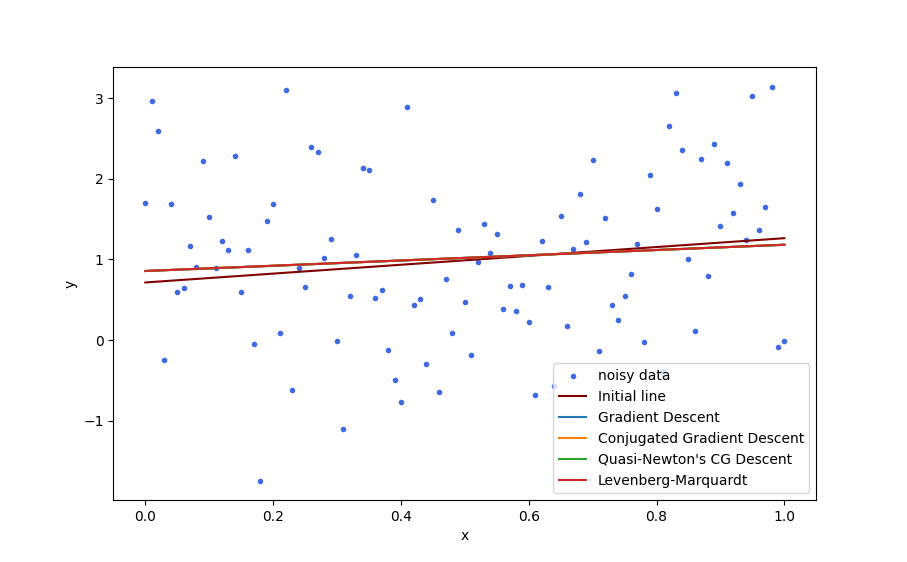
\includegraphics[width=\textwidth]{line.png}
\caption{Results of applying Gradient Descent, Conjugated Gradient Descent, Quasi-Newton's Method and Levenberg-Marquardt Algorithm to solve the problem of linear approximation.}
\end{figure}

\newpage

Those methods were again applied to solve the problem of rational approximation. Obtained data is presented below:
\begin{center}
\begin{tabular}{cccc}
\hline
alg/param                   & (A, B)            & Iterations & Function calls \\ \hline
Gradient Descent            & (0.7521, -0.4651) & 20         & 40             \\
Conjugated Gradient Descent & (0.7521, -0.4650) & 10         & 75             \\
Quasi-Newton's Method       & (0.7442, -0.4750) & 10         & 12             \\
Levenberg-Marquardt         & (0.7522, -0.4647) & 32         & 32             \\ \hline
Exhaustive Search (Task 2)  & (1.0000, 0.0000)  & 1000000    & 1000000        \\
Gauss Search (Task 2)       & (1.0000, 0.0000)  & 50         & 144            \\
Nelder-Mead Search (Task 2) & (0.7522, -0.4647) & 39         & 76             \\ \hline
\end{tabular}
\end{center}
Due to non-linearity, methods of Exhaustive Search and Gauss Search converged to a minimum, different from all other methods, providing similar results (additionally, Quasi-Newton's Method diverged from the others). In terms of performance, again, methods utilizing derivatives converged significantly faster (taking only 10 to 32 iterations and up to 40 function calls) which contrasts slow direct methods.

\begin{figure}[!h]
\centering
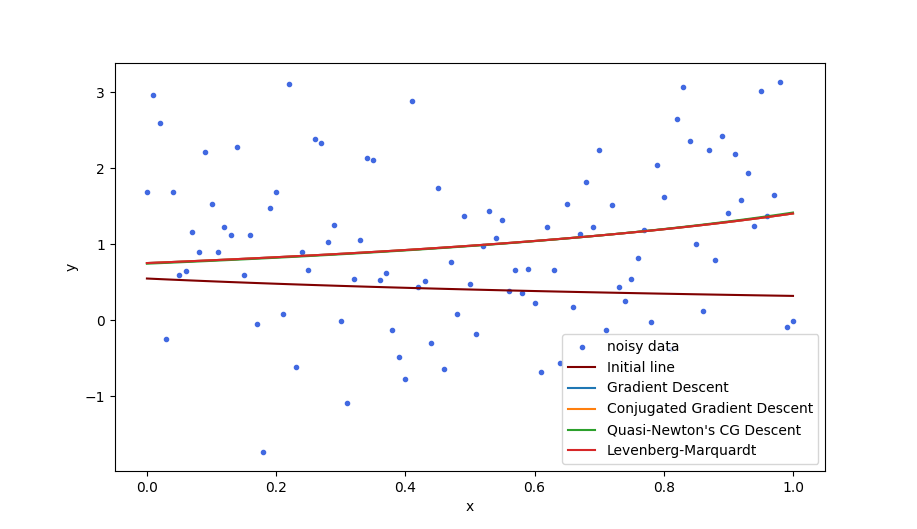
\includegraphics[width=\textwidth]{rational.png}
\caption{Results of applying Gradient Descent, Conjugated Gradient Descent, Quasi-Newton's Method and Levenberg-Marquardt Algorithm to solve the problem of rational approximation.}
\end{figure}

\section*{Conclusions}
\addcontentsline{toc}{section}{Conclusions}

First- and second-order optimization method such as Gradient Descent, Conjugated Gradient Descent, Quasi-Newton's Method and Levenberg-Marquardt Algorithm were applied to tasks of unconstrained nonlinear optimization, tested against each other and direct methods and compared in terms of perfomance.

\newpage

\section*{Appendix}
\addcontentsline{toc}{section}{Appendix}

GitHub link: \url{https://github.com/Dormant512/itmo_lab_listings/blob/main/lab3.py}.

\begin{figure}[!h]
\centering

\includegraphics[width=0.3\textwidth]{lab3.png}
\end{figure}


\end{document}
